\documentclass[aspectratio=169]{beamer}
%[handout]

\usetheme[progressbar=frametitle]{metropolis}
\usepackage{appendixnumberbeamer}

\usepackage[utf8]{inputenc}
\usepackage[T1]{fontenc}

\usepackage[brazil]{babel}
\usepackage[outputdir=..]{minted}
\usepackage{xcolor}
\usepackage{soul} % strikethrough
\usepackage{advdate}
\usepackage{graphicx}
\graphicspath{{figs/}}
\usepackage{graphbox}

\usepackage[ampersand]{easylist}

\usepackage{multirow}
\usepackage{multicol}
\usepackage{subcaption}

\usepackage{pgf,tikz}
\usetikzlibrary{shapes,arrows,positioning}
\usetikzlibrary{circuits.logic.US}
\usetikzlibrary{matrix,calc}

\usepackage{karnaugh-map}

\usepackage{pgfpages}
\setbeameroption{hide notes} % Only slides
% \setbeameroption{show only notes} % Only notes
% \setbeameroption{show notes on second screen=right} % Both

% \graphicspath{{../figs/}}

\definecolor{bgc}{rgb}{0.95,0.9,0.95}
\definecolor{links}{HTML}{2A7F7F}
\hypersetup{colorlinks,linkcolor=,urlcolor=links}

\newminted{verilog}{fontsize=\scriptsize, 
    linenos,
    numbersep=8pt,
    bgcolor=bgc,
    tabsize=4,
    framesep=3mm} 
    %frame=lines,

\newcommand{\verilog}[1]{\verilogf{#1}{\footnotesize}}

\newcommand{\verilogf}[2]{\inputminted[fontsize=#2, 
    linenos,
    tabsize=2,
    numbersep=4pt,
    bgcolor=bgc,
    framesep=3mm]{verilog}{../codes/#1.v}
}

\newminted{nasm}{fontsize=\scriptsize, 
		   linenos,
		   numbersep=8pt,
           bgcolor=bgc,
		   framesep=3mm} 

\usepackage{booktabs}
\usepackage[scale=2]{ccicons}

\usepackage{pgfplots}
\usepgfplotslibrary{dateplot}

\usepackage{hyperref}


\usepackage{xspace}
\newcommand{\themename}{\textbf{\textsc{metropolis}}\xspace}



\usepackage{pifont}% http://ctan.org/pkg/pifont
\newcommand{\cmark}{\ding{51}}%
\newcommand{\xmark}{\ding{55}}%

% \tiny	
% \scriptsize
% \footnotesize
% \small	
% \normalsize	
% \large	
% \Large	
% \LARGE	
% \huge	
% \Huge	



\newminted{python}{fontsize=\scriptsize, 
		   linenos,
		   breaklines,
		   numbersep=8pt,
           tabsize=2,
		   framesep=3mm} 
		   
\newminted{verilog}{fontsize=\scriptsize, 
		   linenos,
		   breaklines,
		   numbersep=8pt,
           tabsize=2,
		   framesep=3mm} 
		   




\definecolor{bgc}{rgb}{0.95,0.9,0.95}
\definecolor{links}{HTML}{2A7F7F}
\hypersetup{colorlinks,linkcolor=,urlcolor=links}


% \usepackage[style=apa]{biblatex}
% \addbibresource{mm.bib}


% \author{\large Prof. Ricardo Menotti (\href{mailto:menotti@ufscar.br}{menotti@ufscar.br})}

\newcommand{\newauthor}[2]{
  \parbox{0.50\textwidth}{
    \texorpdfstring
      {
        \centering
        \small #1 \newline
        {\scriptsize{\urlstyle{same}\href{mailto:#2}{#2}\urlstyle{tt}}}
      }
      {#1} \newline
  }
}

\author{
  \newauthor{Prof. Ricardo Menotti}{menotti@ufscar.br}
\and \newauthor{Prof. Luciano de Oliveira Neris}{lneris@ufscar.br}  
%\and \newauthor{Prof. Artino Quintino da Silva Filho}{artino@ufscar.br}
% \and \newauthor{Prof. Maurício Figueiredo}{mauricio@ufscar.br}
% \and \newauthor{Prof. Edilson Kato}{kato@ufscar.br}
% \and \newauthor{Prof. Roberto Inoue}{rsinoue@ufscar.br}
}

\date{Atualizado em: \today}

\institute{\large \textbf{Departamento de Computação} \\
Centro de Ciências Exatas e de Tecnologia \\
Universidade Federal de São Carlos}

\title{Lógica Digital (1001351)}

\titlegraphic{\hfill
\includegraphics[height=1.5cm]{LogoUfscar}}



\subtitle{Outros Circuitos Combinacionais} % 

\begin{document}

\begin{frame}
	\titlepage
\end{frame} 

% \begin{frame}
%         \tableofcontents[pausesections]
% \end{frame} 

\section{Comparadores}

\begin{frame}{Comparador}   \centering
    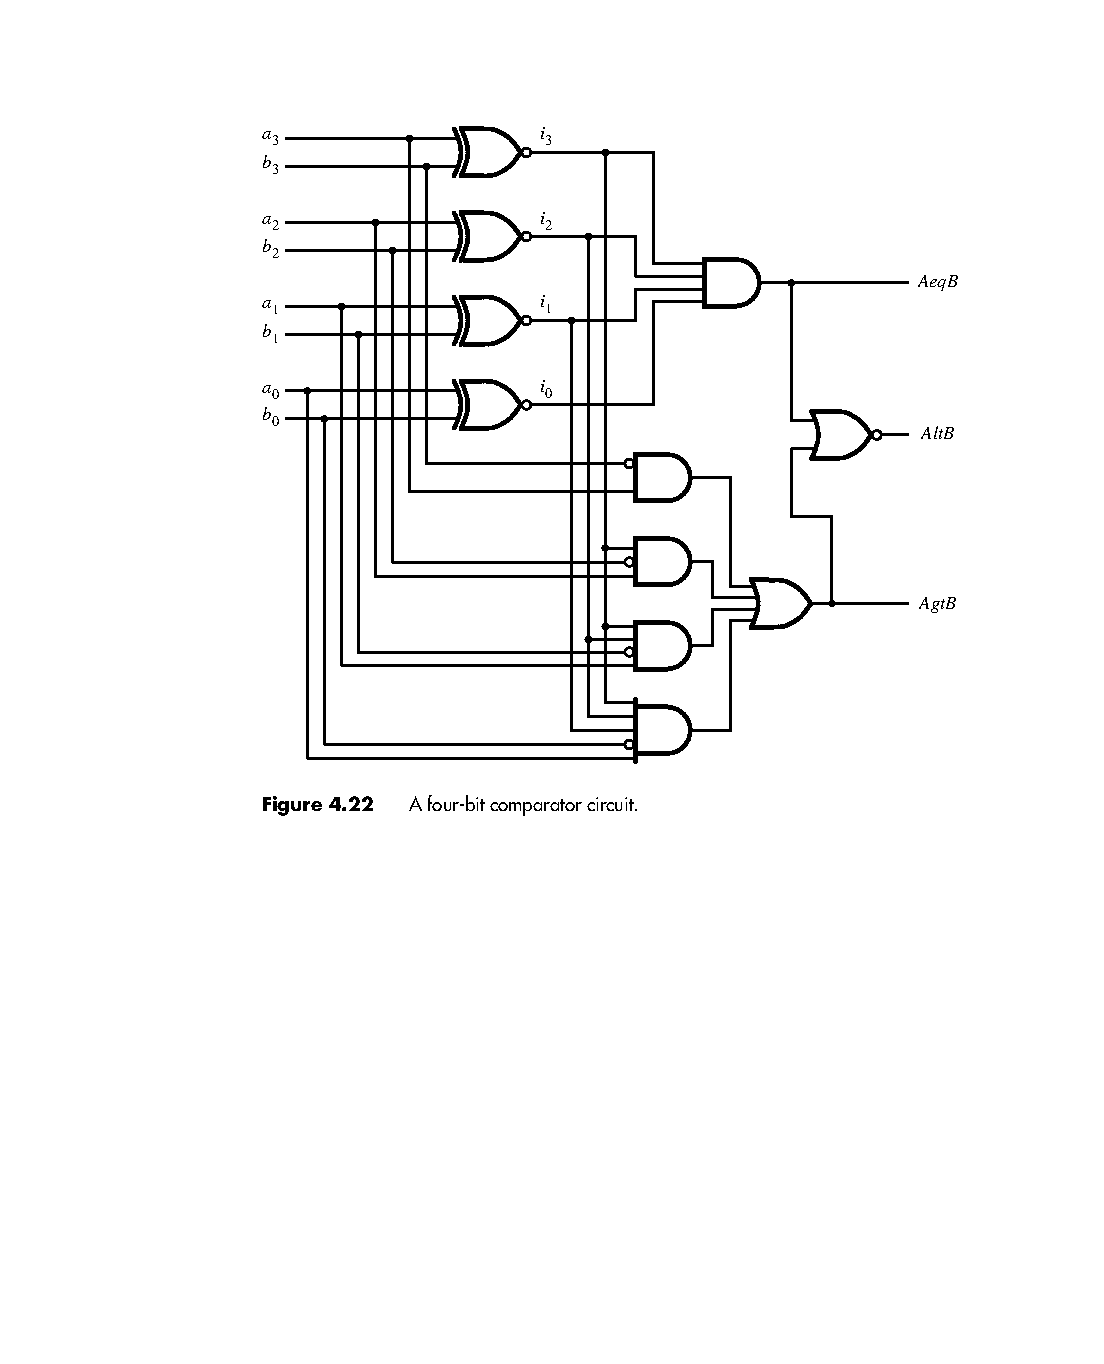
\includegraphics[width=.55\textwidth]{VerilogFig4_22} \\
\end{frame}

\begin{frame}[fragile]{figure4.40.v}
    \verilogf{figure4.40}{\scriptsize}
\end{frame} 

\begin{frame}{Comparador por subtração}   \centering
    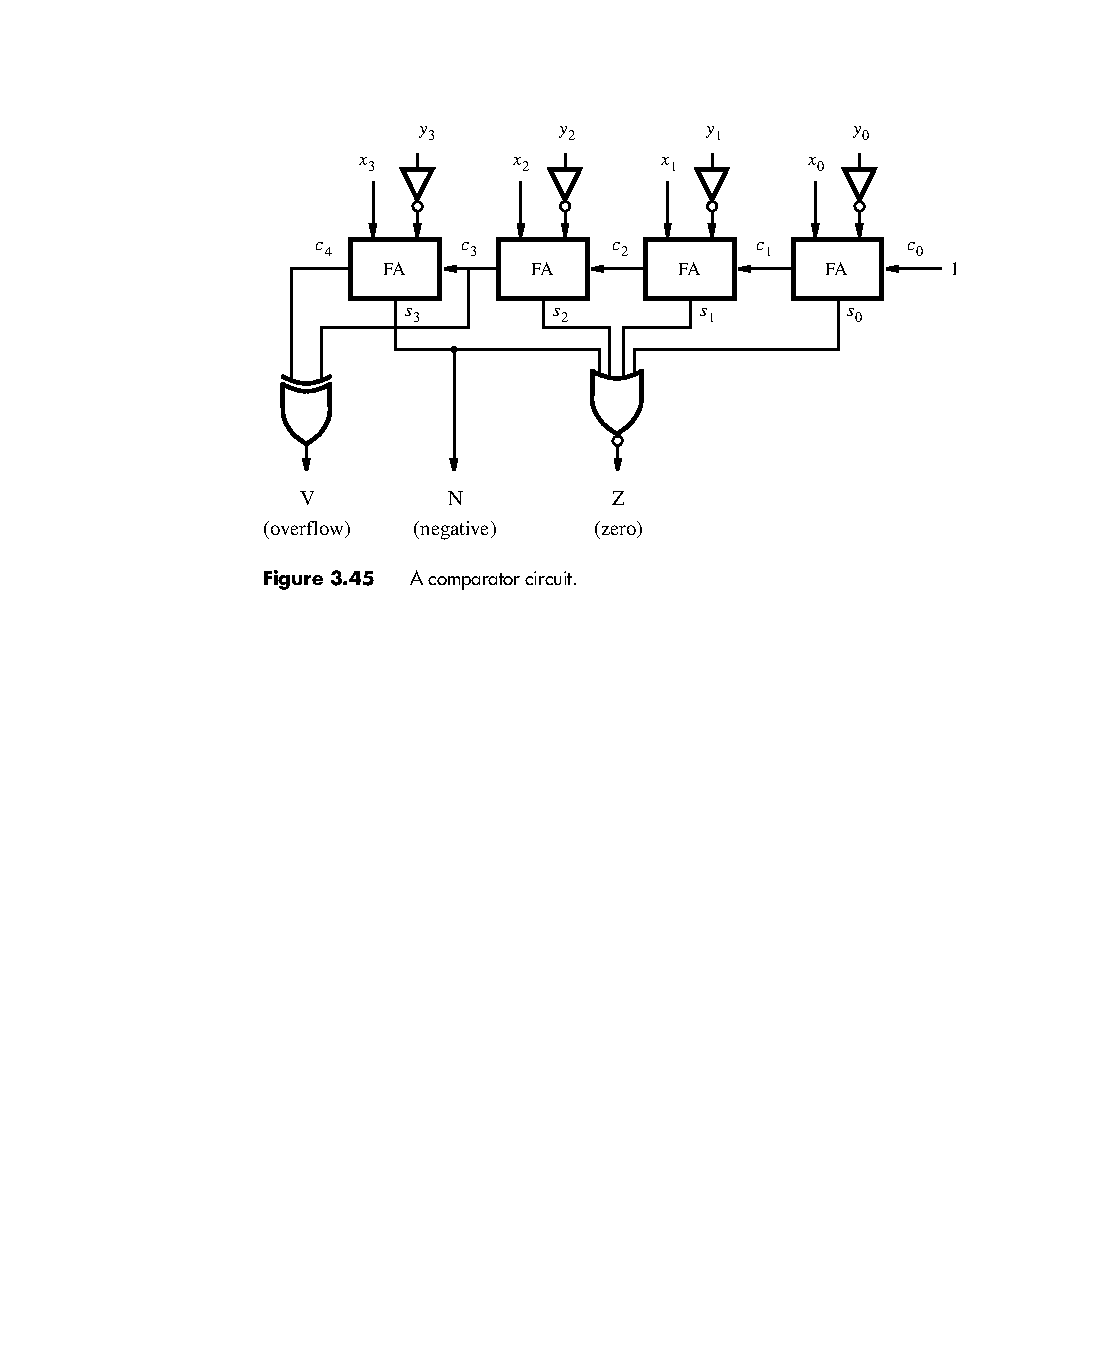
\includegraphics[width=.9\textwidth]{VerilogFig3_45} \\
    \scriptsize $X<Y \iff N \oplus V$ \hfill $X=Y \iff Z$ \hfill $X\leq Y \iff (N \oplus V) + Z$
\end{frame}

\begin{frame}[fragile]{figure3.46.v}
    \verilogf{figure3.46}{\tiny}
\end{frame} 

\begin{frame}[fragile]{figure3.47.v}
    \verilogf{figure3.47}{\tiny}
\end{frame} 

\section{Deslocadores}

\begin{frame}{Deslocamento (\textit{shift})} \centering
    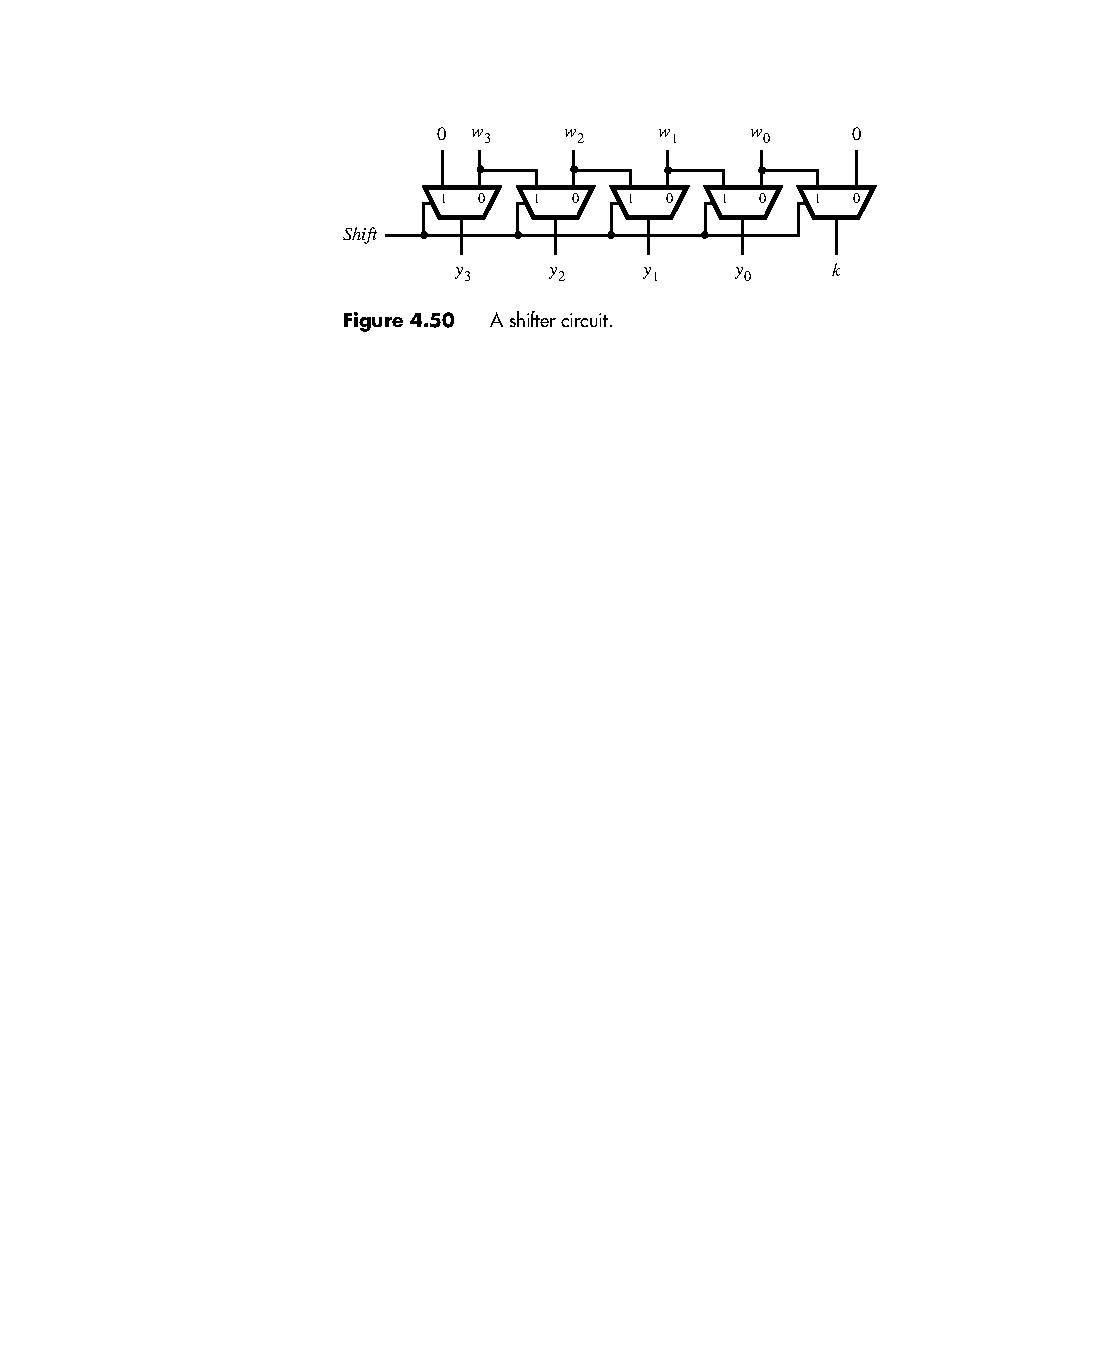
\includegraphics[width=.75\textwidth]{VerilogFig4_50}
\end{frame}

\begin{frame}[fragile]{figure4.53.v}
    \verilogf{figure4.53}{\tiny}
\end{frame} 

\begin{frame}[fragile]{figure4.54.v}
    \verilogf{figure4.54}{\tiny}
\end{frame} 

\begin{frame}{Deslocamento (\textit{rotate})} \centering
    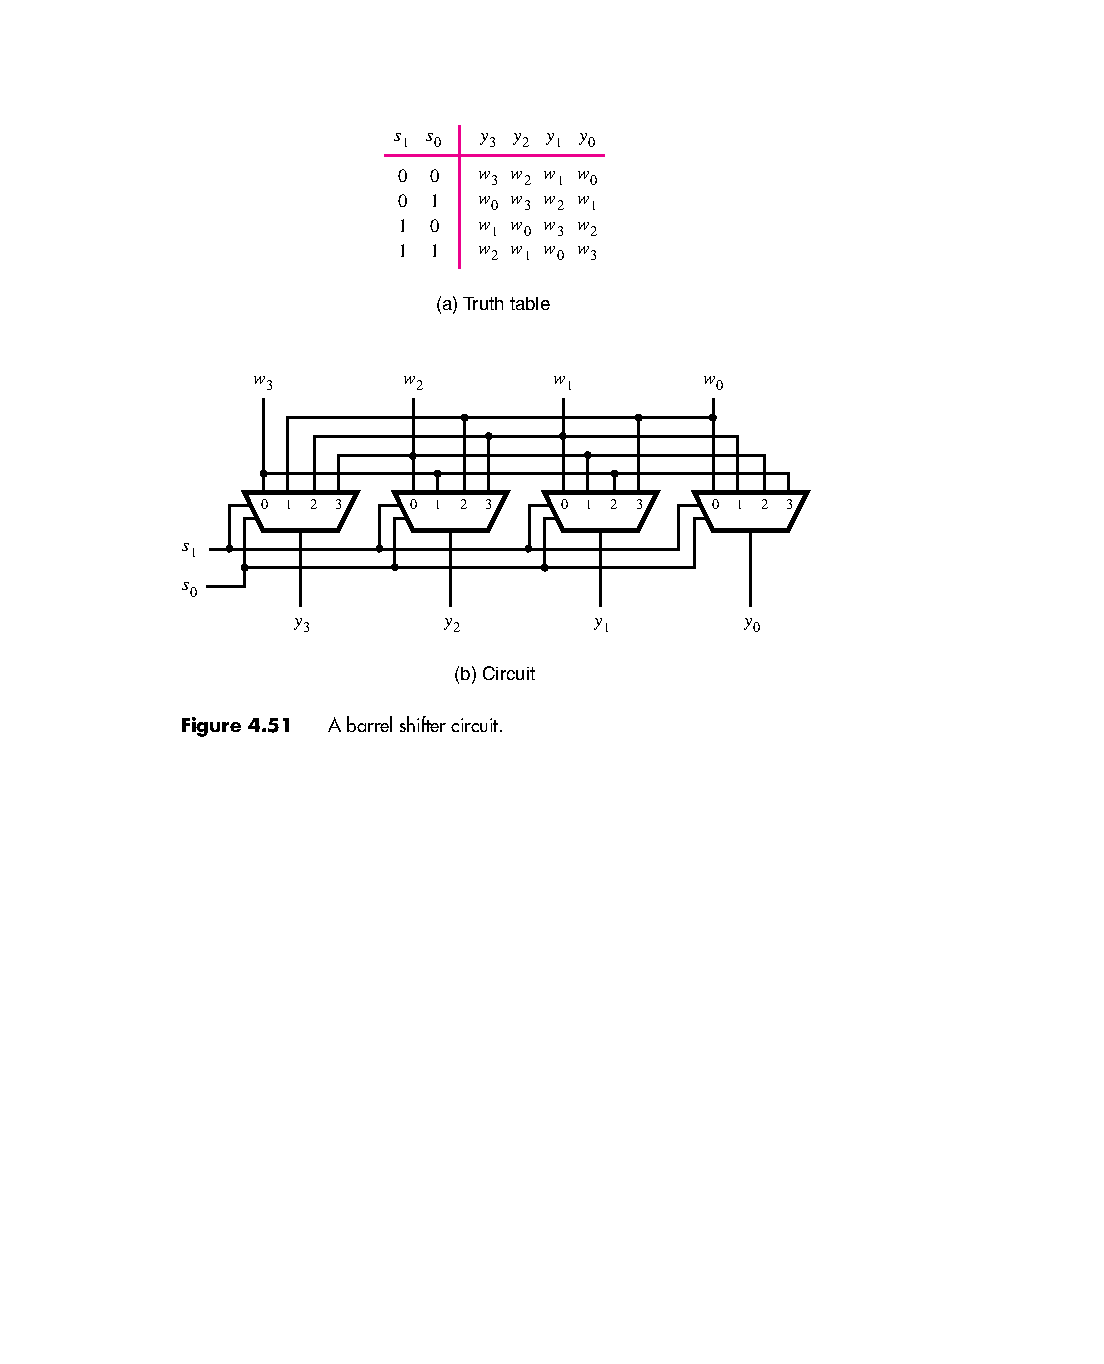
\includegraphics[width=.55\textwidth]{VerilogFig4_51}
\end{frame}

\begin{frame}[fragile]{figure4.55.v}
    \verilogf{figure4.55}{\scriptsize}
\end{frame} 

\section{ULA}

\begin{frame}{ULA}
    \begin{columns}
        \begin{column}{0.40\textwidth} \centering
            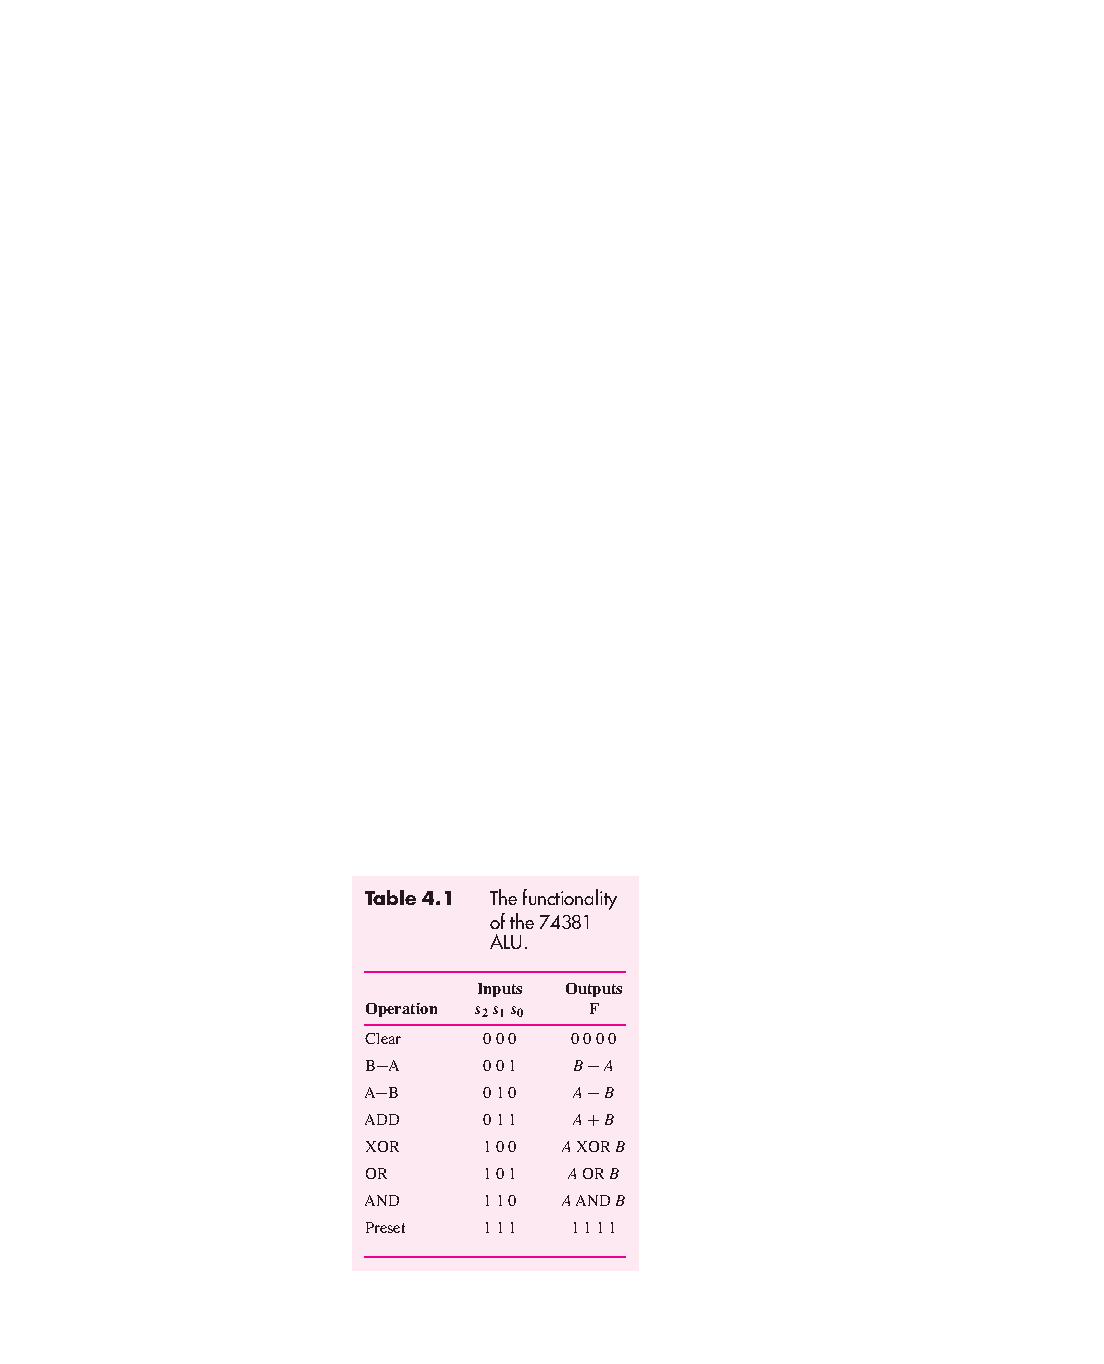
\includegraphics[width=\textwidth]{VerilogTab4_1} 
        \end{column}
        \pause
        \begin{column}{0.60\textwidth}
            \verilogf{figure4.35}{\scriptsize}
        \end{column}    
    \end{columns}    
\end{frame}

\section{Verilog}

\begin{frame}{Operadores em Verilog (1/2)} \centering
    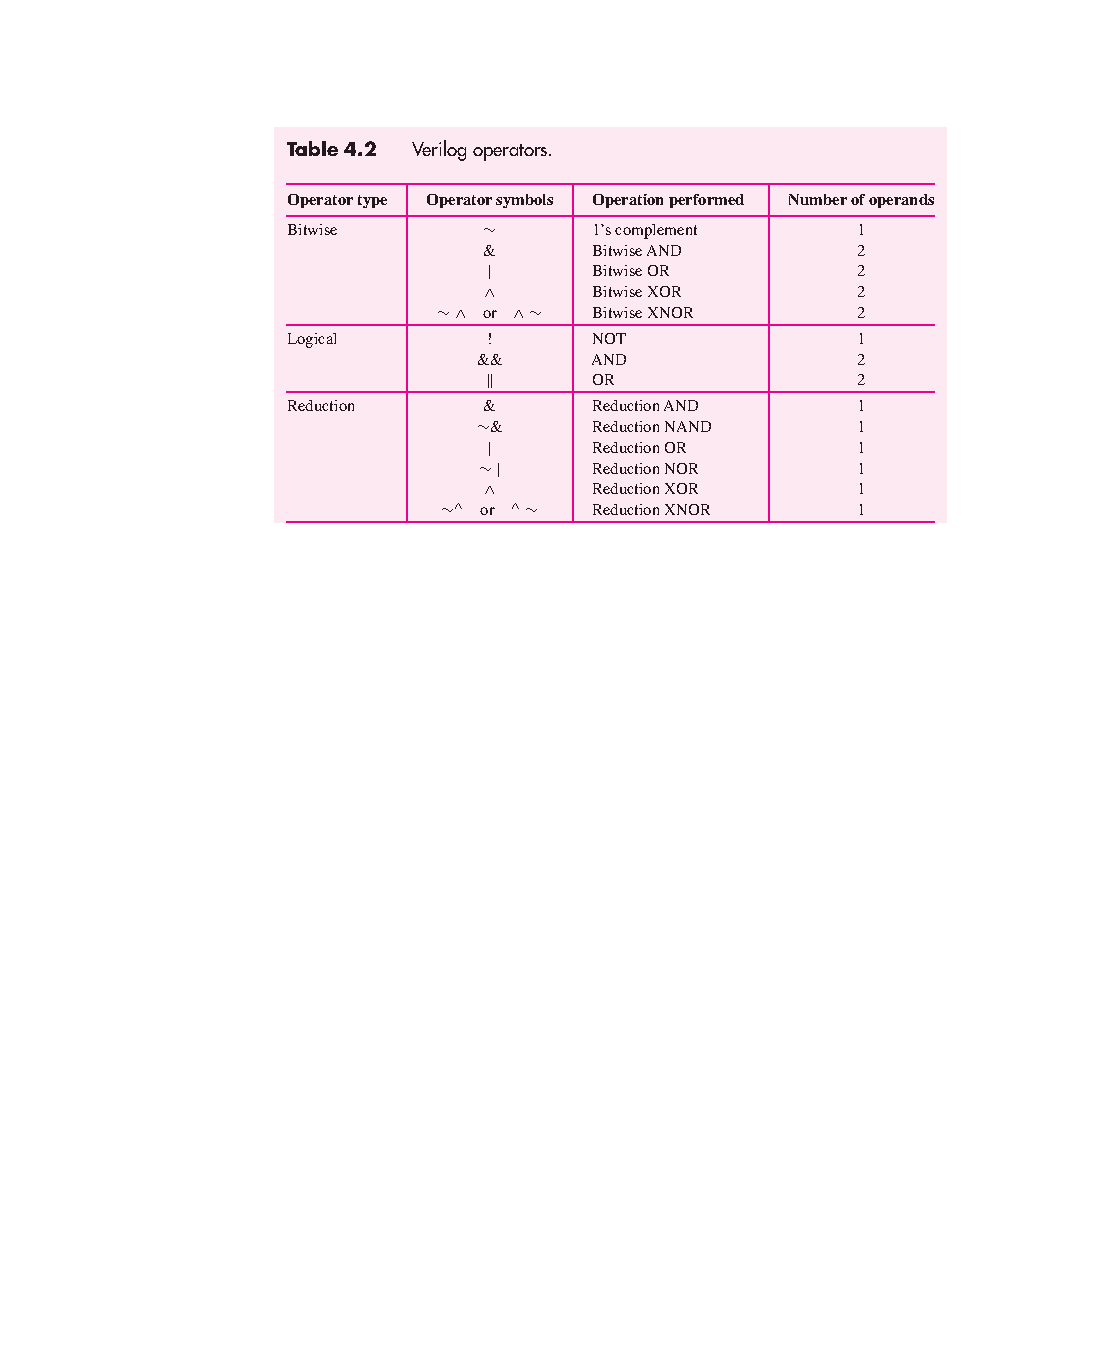
\includegraphics[width=.9\textwidth]{VerilogTab4_2a} \\
    . . .
\end{frame}

\begin{frame}{Operadores em Verilog (2/2)} \centering
    . . . \\ 
    \vspace{0.3cm}
    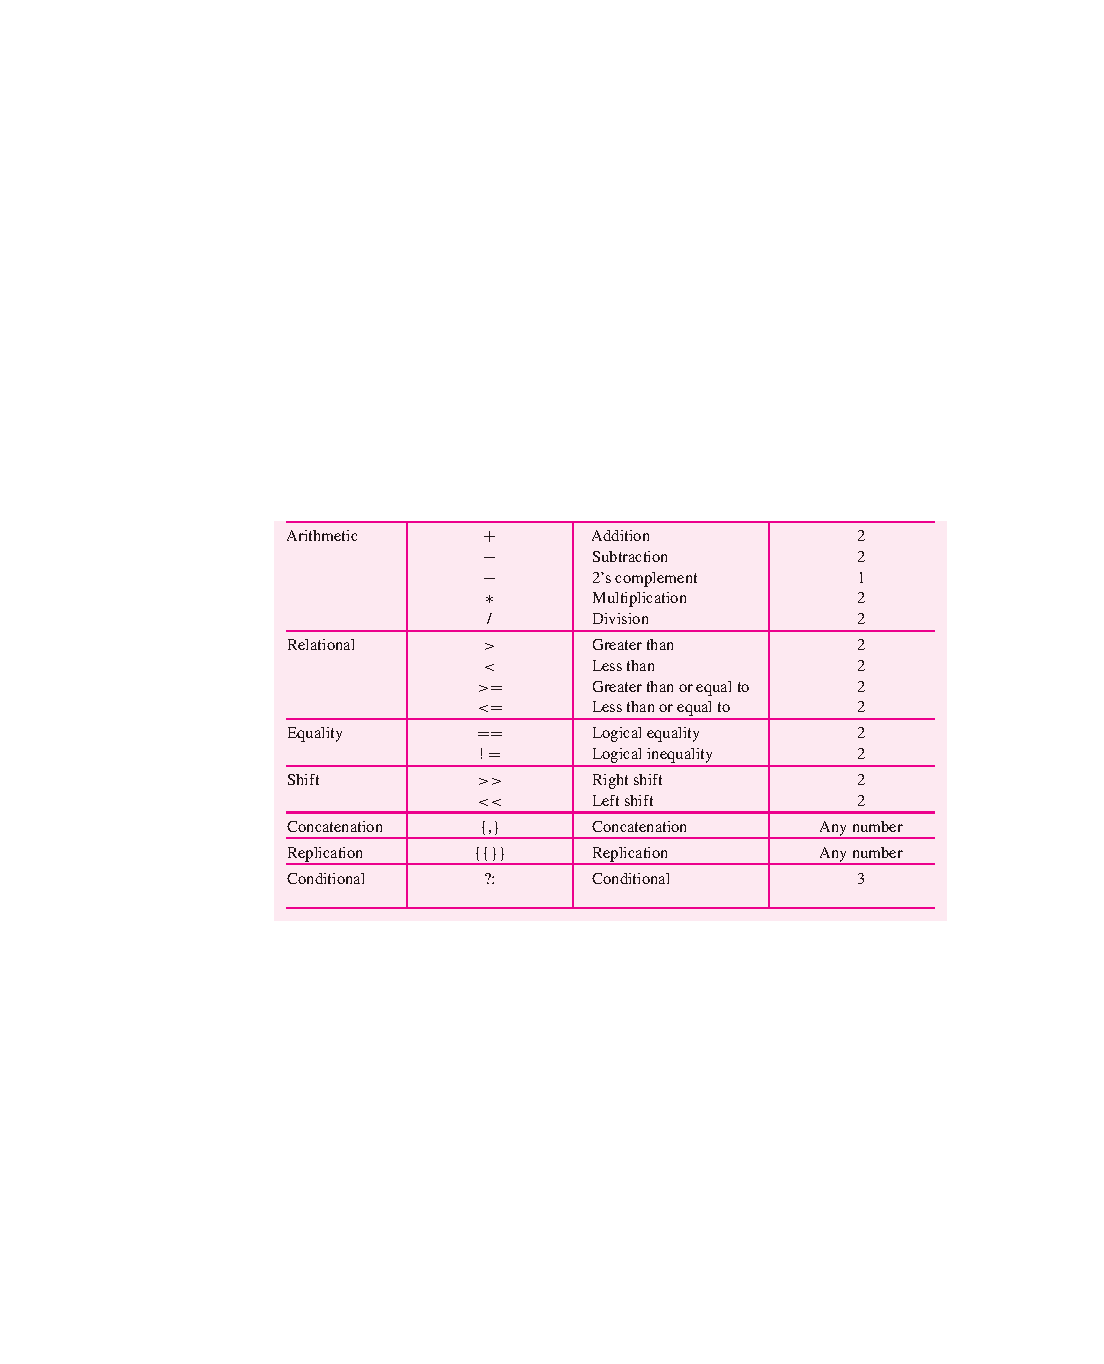
\includegraphics[width=.9\textwidth]{VerilogTab4_2b} 
\end{frame}

\begin{frame}{Precedencia dos Operadores em Verilog} \centering
    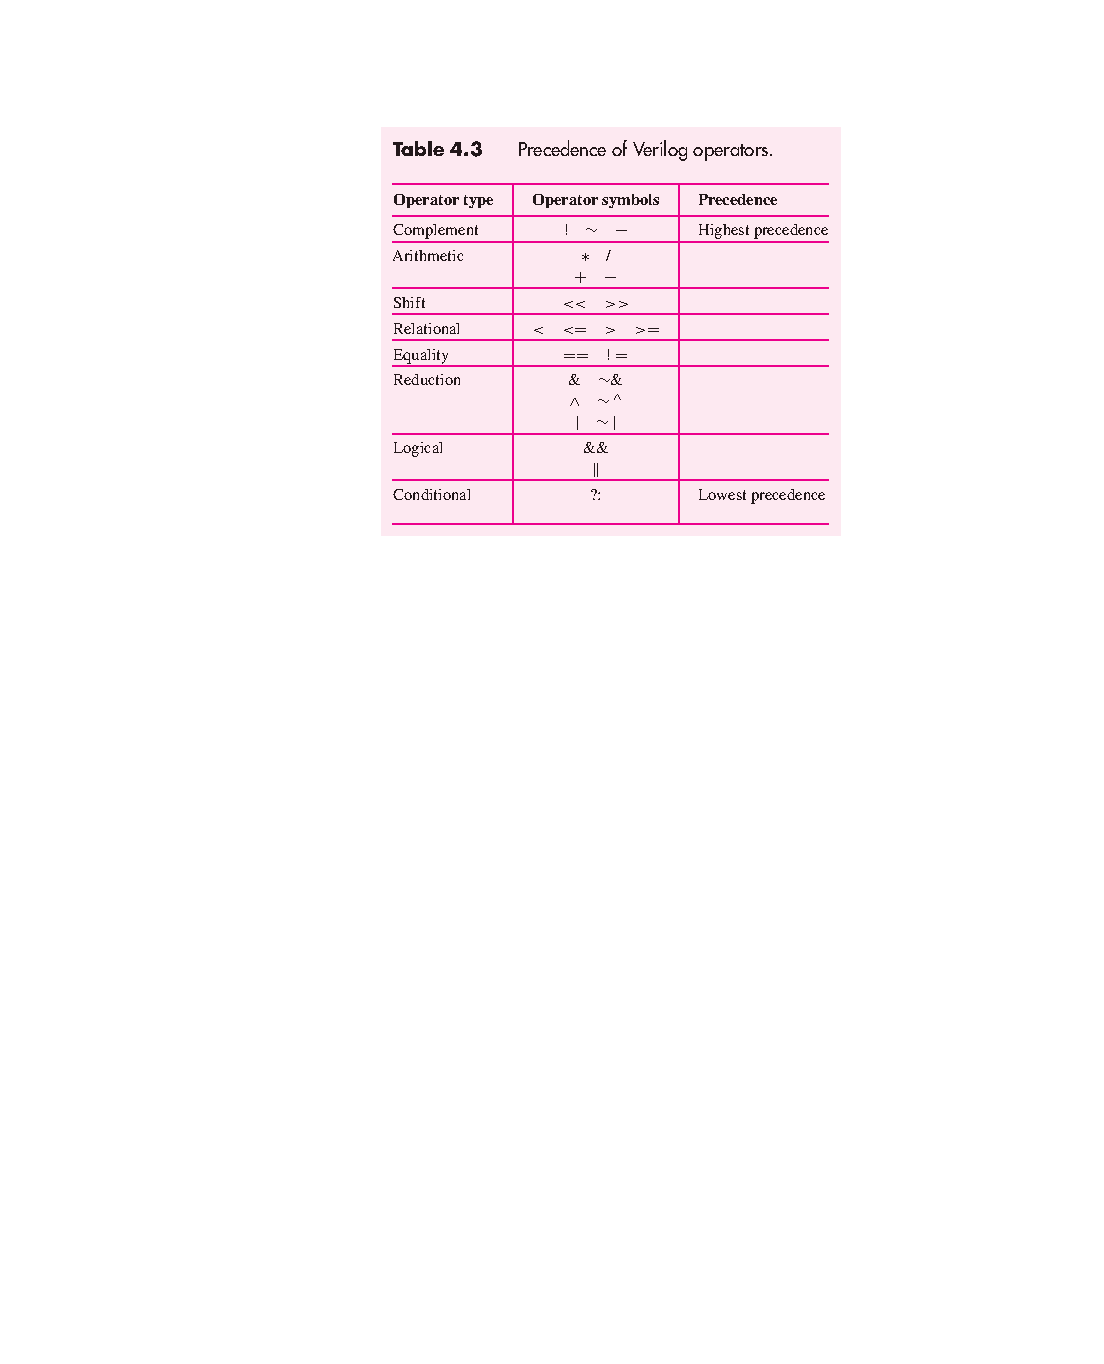
\includegraphics[width=.6\textwidth]{VerilogTab4_3} 
\end{frame}

\section{Erros comuns}

\begin{frame}[fragile]
	\frametitle{Perigo!: Especificação Incompleta}
	\begin{columns}
        \column{0.4\textwidth}
        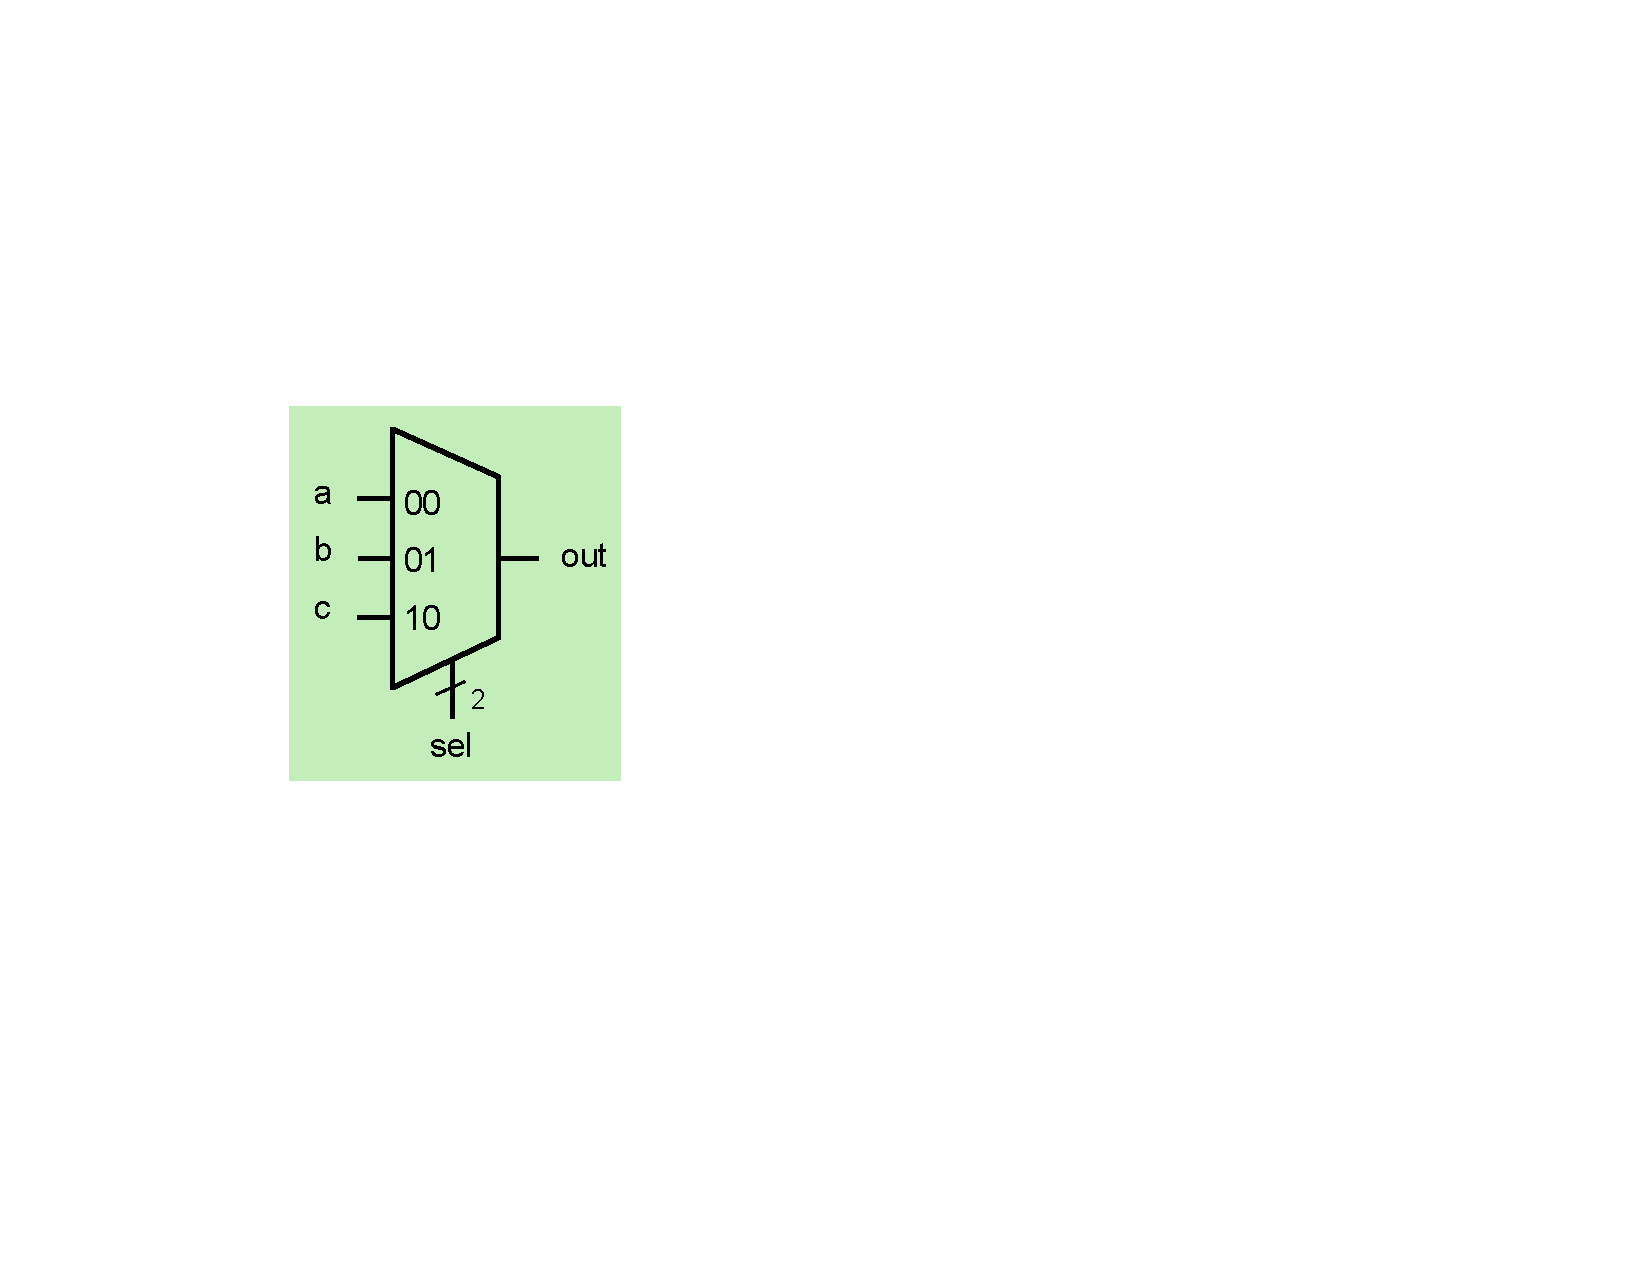
\includegraphics[scale=.5]{figs/Mux3to1}
        \column{0.6\textwidth}
	    \begin{verilogcode}
module mux3to1(a, b, c, sel, out);
  input [1:0] sel;
  input a, b, c;
  output out;
  reg out;
  
  always @(a or b or c or sel)
  begin
    case (sel)
      2'b00: out = a;
      2'b01: out = b;
      2'b10: out = c;
    endcase
  end
endmodule
        \end{verilogcode}
    \end{columns}
\end{frame}

\begin{frame}[fragile]
	\frametitle{Perigo!: Especificação Incompleta}
    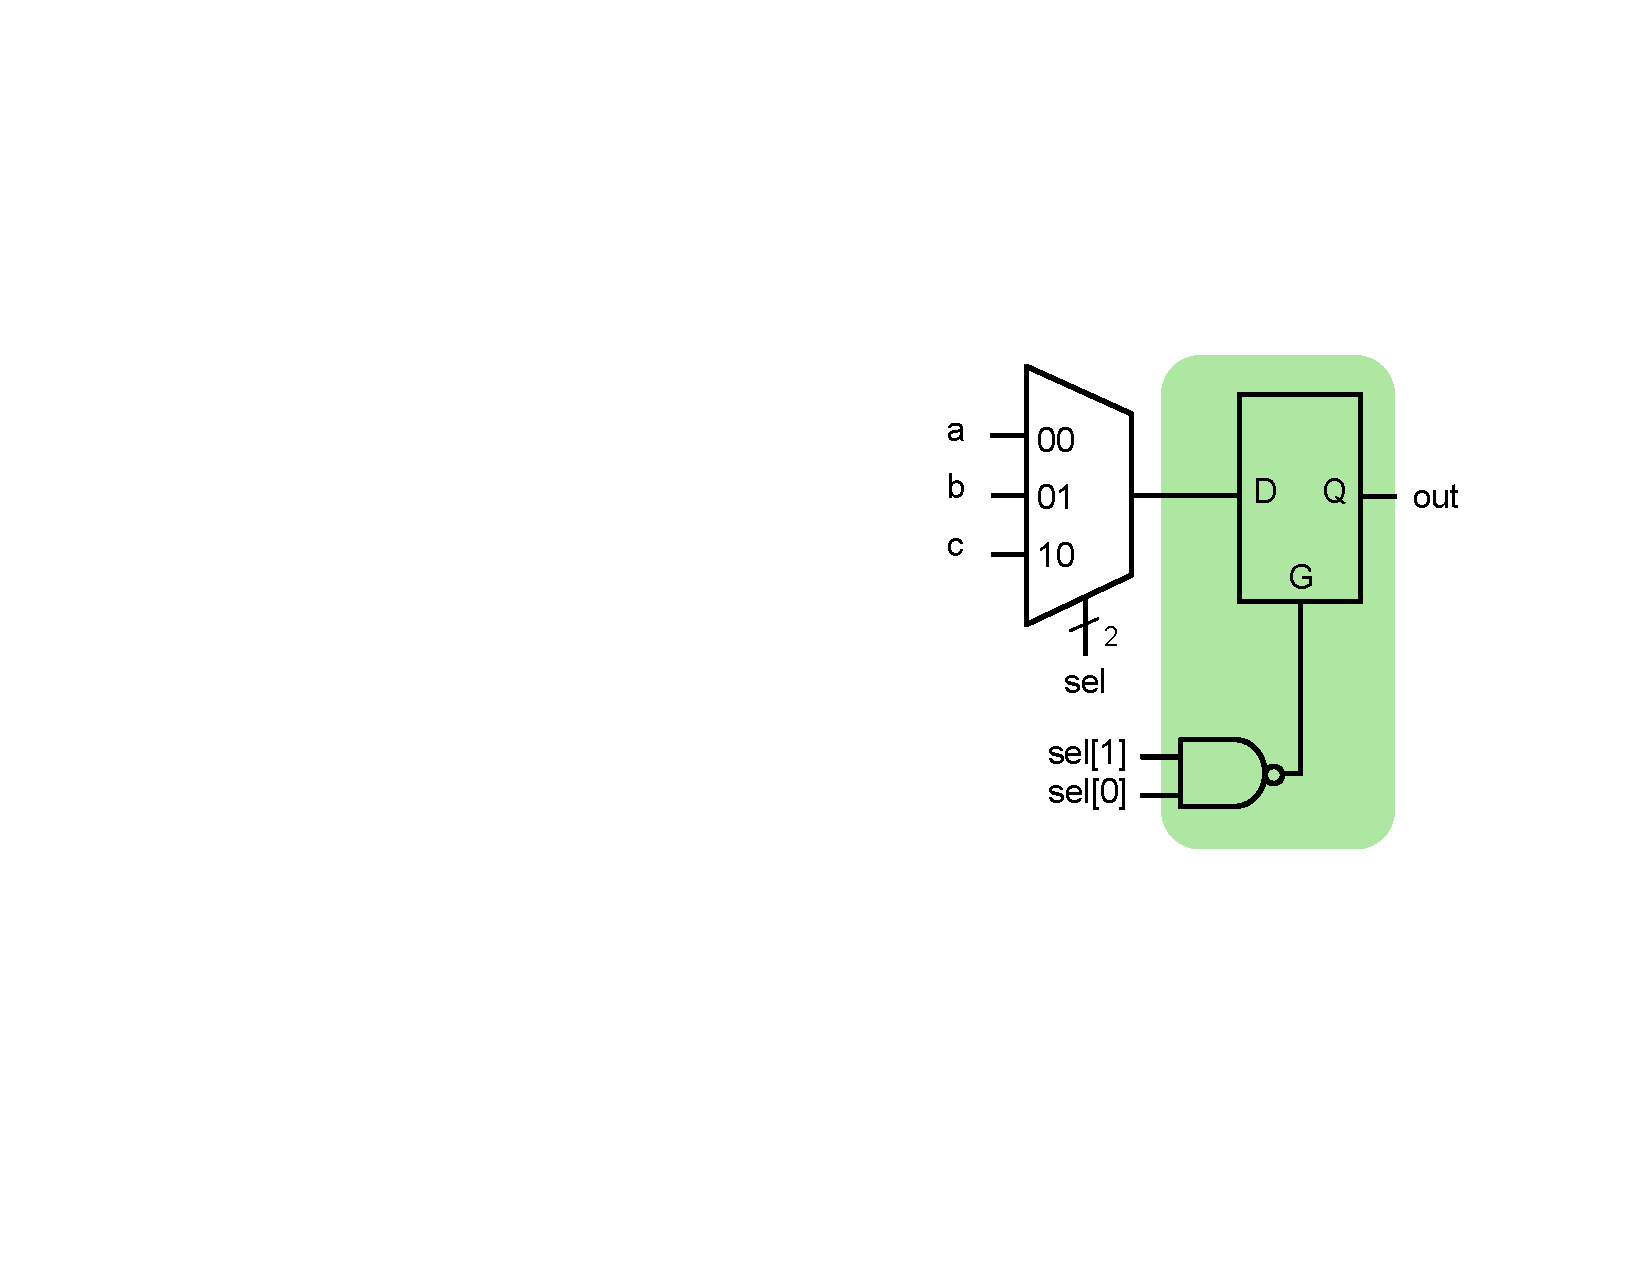
\includegraphics[scale=.5]{figs/Mux3to1Latch}
\end{frame}

\begin{frame}[fragile]
	\frametitle{Evitando a Especificação Incompleta}
 \begin{multicols}{2}
	\begin{verilogcode}
  always @(a or b or c or sel)
  begin
    out = 1'bx
    case (sel)
      2'b00: out = a;
      2'b01: out = b;
      2'b10: out = c;
    endcase
  end
    \end{verilogcode}
	\begin{verilogcode}
  always @(a or b or c or sel)
  begin
    case (sel)
      2'b00: out = a;
      2'b01: out = b;
      2'b10: out = c;
      default: out = 1'bx
    endcase
  end
    \end{verilogcode}
    \end{multicols}
\end{frame}

\begin{frame}[fragile]
	\frametitle{Perigo!: Prioridade Indesejada}
	\begin{columns}
        \column{0.4\textwidth}
        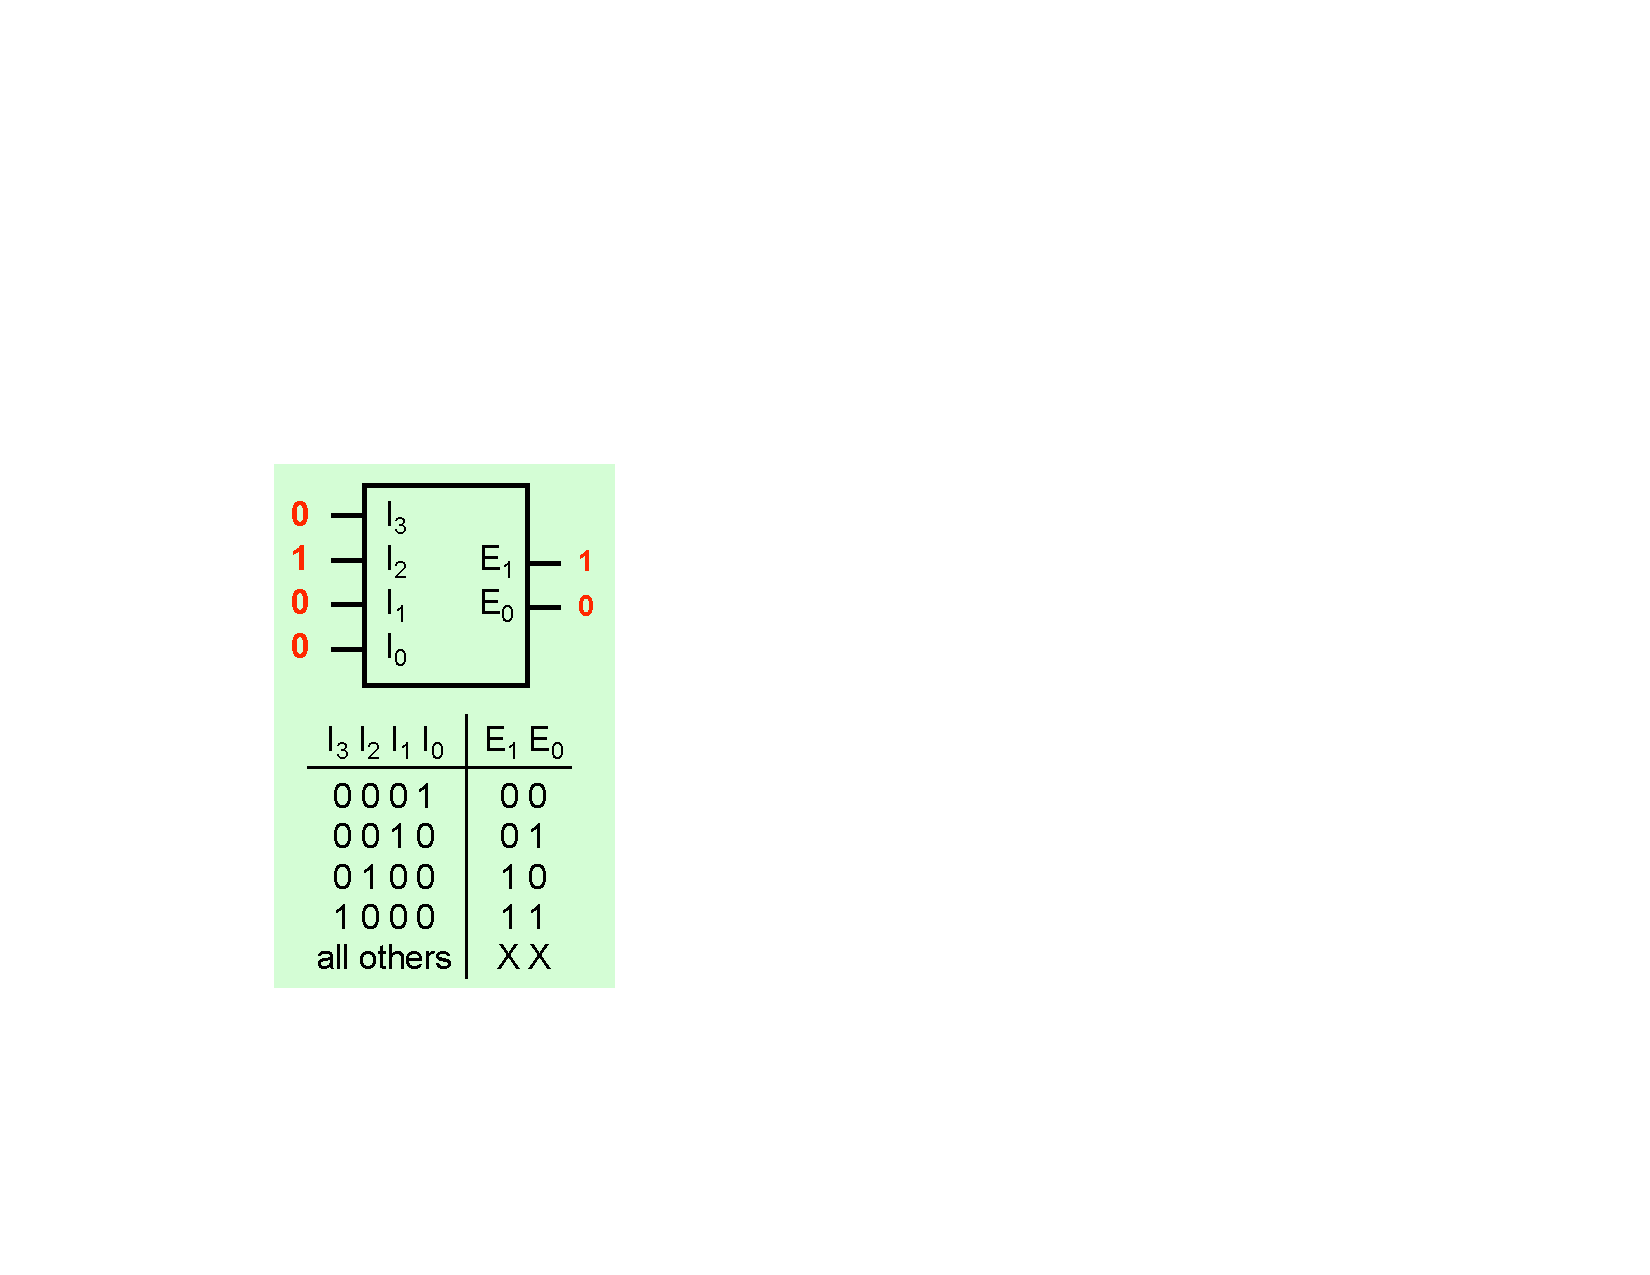
\includegraphics[scale=.5]{Encoder4to2}
        \column{0.6\textwidth}
    	\begin{verilogcode}
module binary_encoder(i, e); 
  input [3:0] i;
  output [1:0] e;
  reg e;
 
  always @(i)
  begin
    if (i[0]) 
      e = 2'b00; 
    else if (i[1]) 
      e = 2'b01; 
    else if (i[2]) 
      e = 2'b10; 
    else if (i[3]) 
      e = 2'b11; 
    else 
      e = 2'bxx;
  end
endmodule
        \end{verilogcode}
    \end{columns}
\end{frame}

\begin{frame}[fragile]
	\frametitle{Perigo!: Prioridade Indesejada}
    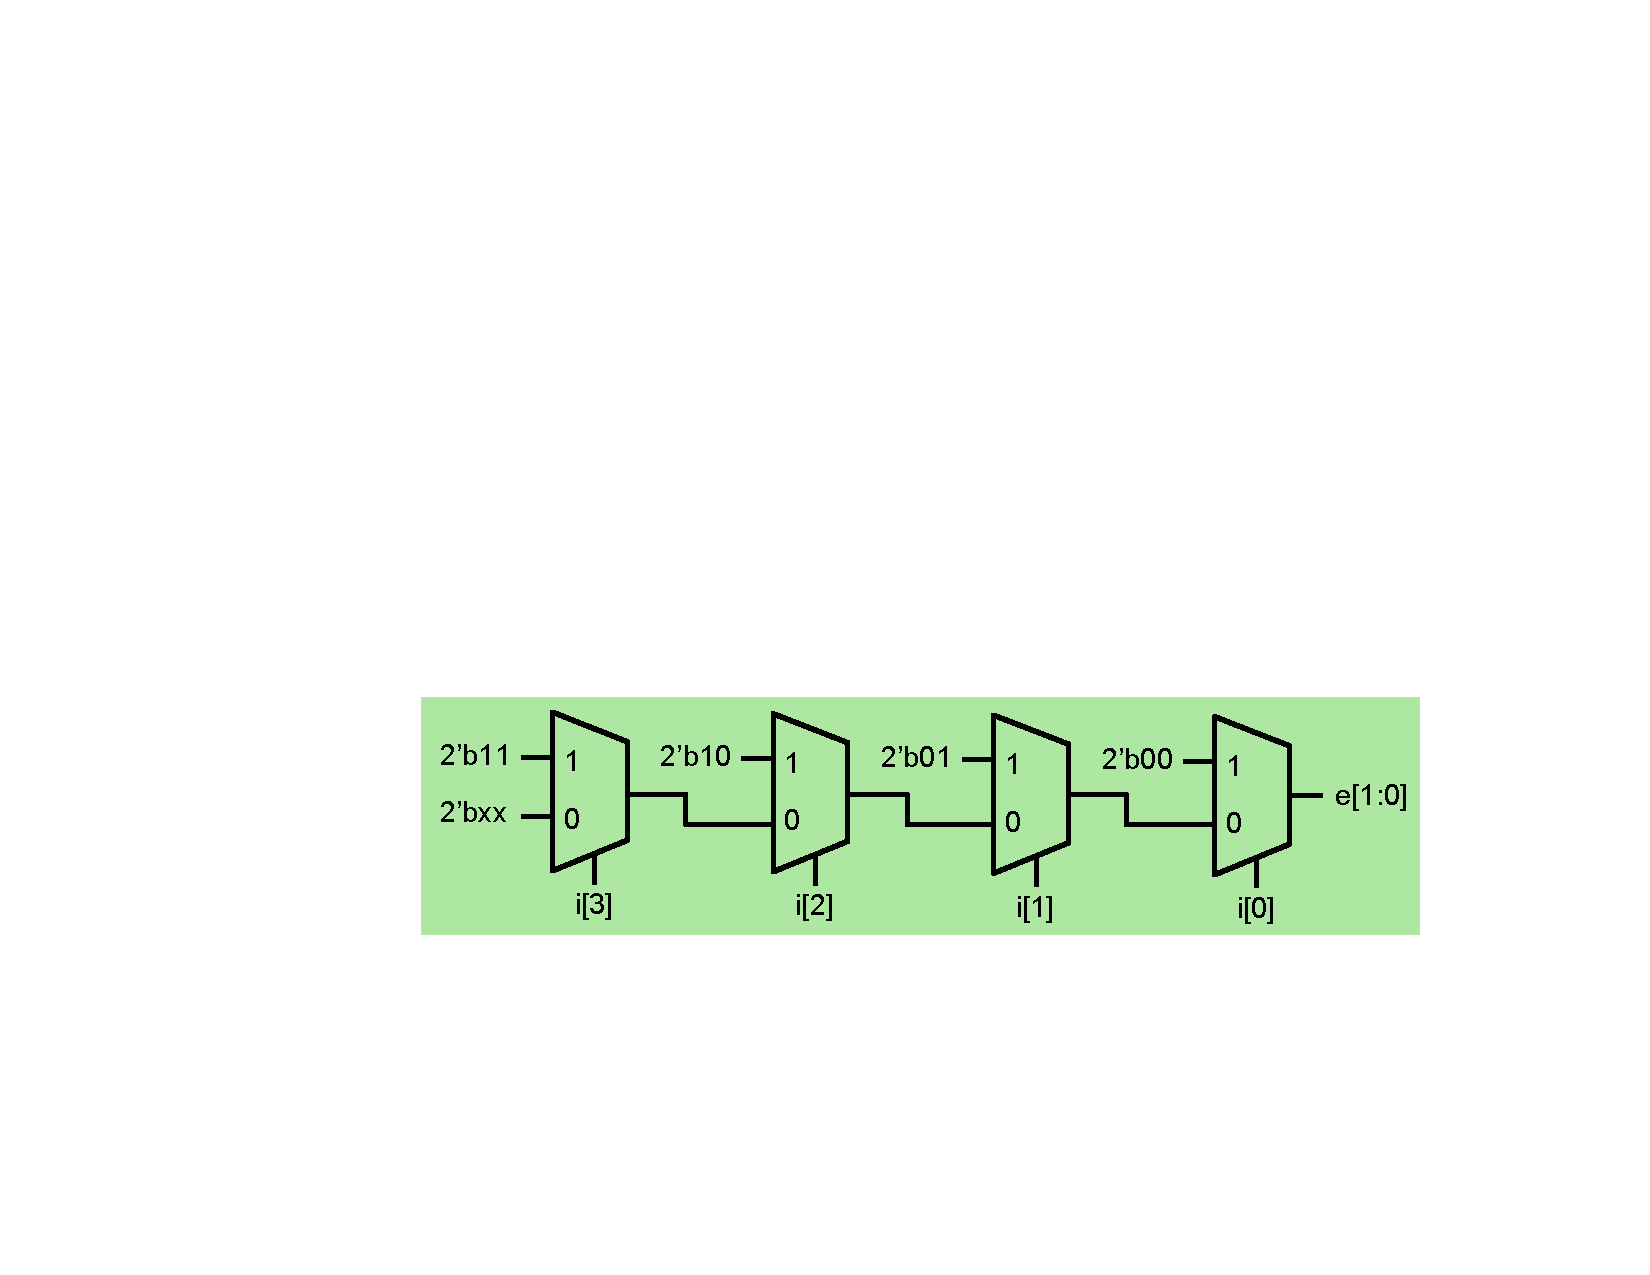
\includegraphics[scale=.5]{figs/Encoder4to2Pri}
\end{frame}

\begin{frame}[fragile]
	\frametitle{Evitando Prioridade Indesejada}
	\begin{columns}
        \column{0.4\textwidth}
        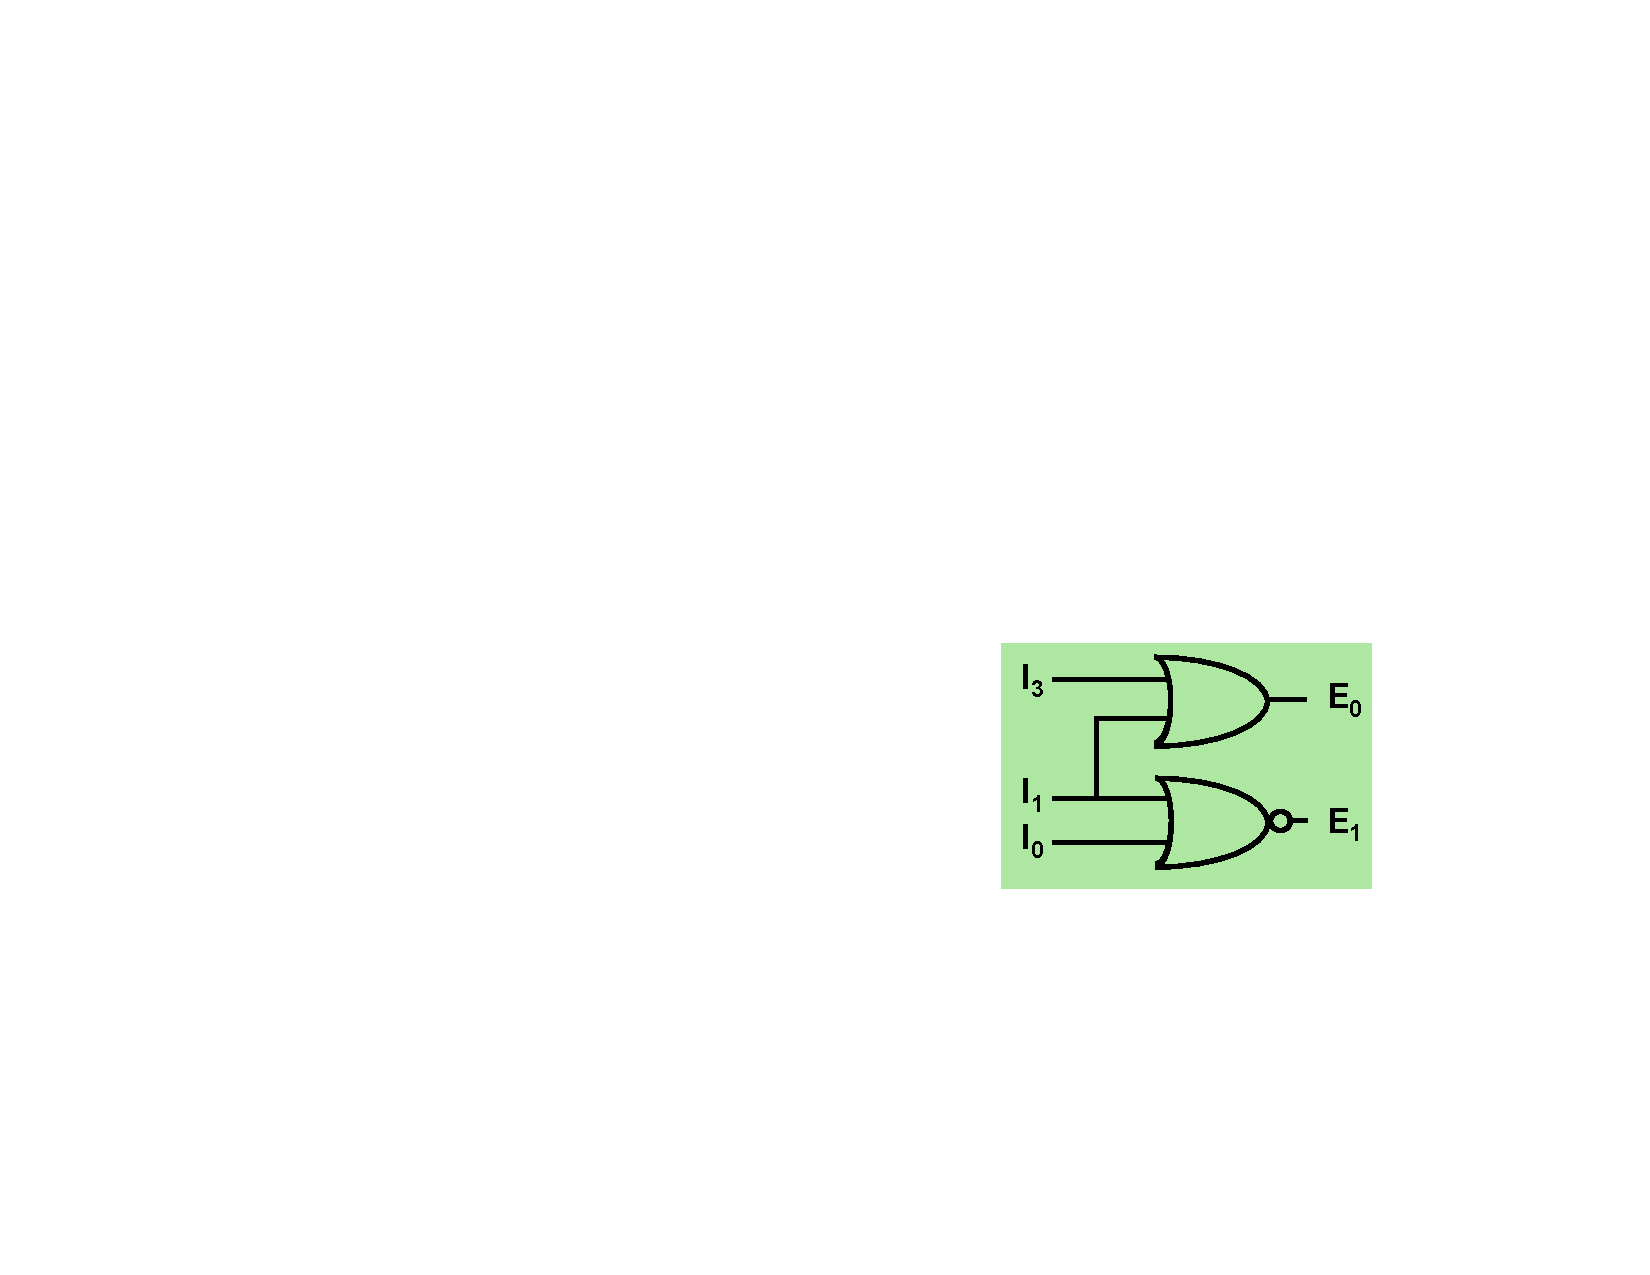
\includegraphics[scale=.5]{figs/Encoder4to2Min}
        \column{0.6\textwidth}
    	\begin{verilogcode}
module binary_encoder(i, e); 
  input [3:0] i;
  output [1:0] e;
  reg e;
 
  always @(i)
  begin
    if (i == 4'b0001) 
      e = 2'b00; 
    else if (i == 4'b0010) 
      e = 2'b01; 
    else if (i == 4'b0100) 
      e = 2'b10; 
    else if (i == 4'b1000) 
      e = 2'b11; 
    else 
      e = 2'bxx;
  end
endmodule
        \end{verilogcode}
    \end{columns}
\end{frame}


\section{Bibliografia} %%%%%%%

\begin{frame}{\insertsection} 
	\begin{itemize}
		\item \href{https://www.google.com.br/search?q=filetype\%3Apdf+Fundamentals+of+Digital+Logic+with+Verilog+Design+&oq=filetype\%3Apdf}{Brown, S. \& Vranesic, Z. - Fundamentals of Digital Logic with Verilog Design, 3rd Ed., Mc Graw Hill, 2009}
	\end{itemize}
\end{frame}

\begin{frame}
	\titlepage
\end{frame} 

\end{document}